\documentclass[elementsmain.tex]{subfiles}
\begin{document}
\section{Hyperplanes and the Row Picture}

We now take up the task of learning to solve systems of linear equations. As a start, we shall be more careful about what one single equation is, and how it may be represented.

\begin{definition}[Linear Equation] A \emph{linear equation the $n$ unknowns $x_1$, $x_2$, \dots, $x_n$} is an equation of the form
\begin{equation}\label{eq:lin-eq}
a_1 x_1 + a_2 x_2 + \dots + a_n x_n = b,
\end{equation}
where each of the $a_i$'s and $b$ are scalars. The scalars $a_i$ are called \emph{coefficients}. Notice that some of the $a_i$'s may be zero, in which case it looks like the corresponding terms are not present. In this case, it may still be necessary to remember that those unknowns matter, depending on the context.

A vector in $R^n$ is said to be a \emph{solution} of the equation when its components, in order, are substituted in for the unknowns $x_i$ the equation becomes true.
\end{definition}


\begin{remark} A linear equation in $n$ unknowns is one that can be rewritten
using the dot product in $\R^n$. In particular, if we write the coefficients in a vector, and the unknowns in a vector like so
\[
N = \begin{pmatrix} a_1 \\ a_2 \\ \vdots \\ a_n\end{pmatrix} \qquad
X = \begin{pmatrix} x_1 \\ x_2 \\ \vdots \\ x_n\end{pmatrix},
\]
then Equation (\ref{eq:lin-eq}) becomes exactly $N\cdot X = b$.
\end{remark} 

\begin{theorem} Let $P$ be a solution to the linear Equation \ref{eq:lin-eq}. 
Then the set of solutions to Equation ($\ref{eq:lin-eq}$) is equal to the the set
\[
\mathcal{S} = \left\{ X\in \R^n \,\middle|\, N \cdot (X- P) = 0 \right\},
\]
where $N$ is the vector of coefficients
\[
N = \begin{pmatrix} a_1 \\ a_2 \\ \vdots \\ a_n\end{pmatrix}.
\]
\end{theorem}

\begin{proof} Fix a solution $P$ to Equation (\ref{eq:lin-eq}):
\[
P = \begin{pmatrix} p_1 \\ p_2 \\ \vdots \\ p_n\end{pmatrix}.
\]
Then by definition we have
\begin{equation}\label{eq:06-1}
N\cdot P = a_1 p_1 + a_2 p_2 + \dots + a_n p_n = b.
\end{equation}

Now, suppose that $X$ is some solution to the equation. Then $N\cdot X=b$, or
\begin{equation}\label{eq:06-2}
N\cdot X = a_1 x_1 + a_2 x_2 + \dots + a_n x_n = b.
\end{equation}
Using the left hand equalities of Equation (\ref{eq:06-1}) and Equation (\ref{eq:06-2}) and doing some rearranging, we see that
\begin{equation*}
\begin{split}
N\cdot X - N\cdot P & = a_1 x_1 + a_2 x_2 + \dots + a_n x_n - \left(a_1 p_1 + a_2 p_2 + \dots + a_n p_n\right) \\
& = a_1(x_1- p_1) + a_2(x_2- p_2) + \dots + a_n(x_n- p_n) \\
& = N \cdot (X-P).
\end{split}
\end{equation*}
But using the right-hand equalities of those equations we see
\[
N\cdot X - N\cdot P = b- b = 0.
\]
So we conclude that if $X$ is a solution to Equation (\ref{eq:lin-eq}), then $N\cdot(X-P)=0$.

Now suppose that $X$ is some vector for which $N\cdot (X-P)=0$. We rearrange the equation like this:
\begin{align*}
N\cdot(X-P) & = 0 \\
N\cdot X - N\cdot P & = 0 \\
N\cdot X & = N\cdot P
\end{align*}
Now we substitute in from the right-hand equality in Equation (\ref{eq:06-1}) and expand out the dot product on the left to see
\[
a_1 x_1 + a_2 x_2 + \dots + a_n x_n = b.
\]
This means that $X$ is a solution of Equation (\ref{eq:lin-eq}).

Since we have proved that an element of $\mathcal{S}$ is a solution of (\ref{eq:lin-eq}) and vice versa. The proof is complete.
\end{proof}

This last theorem connects the idea of the set of solutions to a linear equation to a situation involving a dot product being zero, that is, of orthogonality. The basic picture is like the one in Figure \ref{fig:general-line}. Note the right angle between $X-P$ and $N$ there.

\begin{figure}[h]
\centering
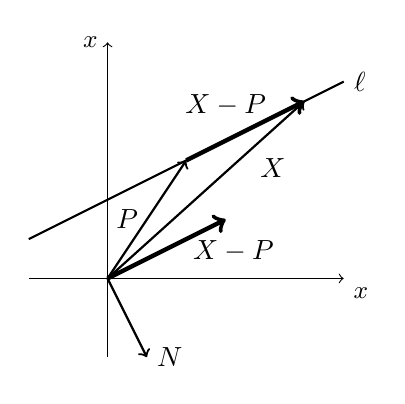
\begin{tikzpicture}[scale=1]
\draw[->] (-1,0) -- (3,0) node[below right] {\small $x$};
\draw[->] (0,-1) -- (0,3) node[left] {\small $x$};
%\draw[thick] (-1,-.5) -- (3,3/2) node[right] {$\ell'$};
\draw[thick,->] (0,0) -- (0.5,-1) node[right] {$N$};
\draw[thick] (-1,.5) -- (3,5/2) node[right] {$\ell$};
\draw[thick,->] (0,0) -- (1,3/2);
\node at (.25,.75) {$P$};
\draw[thick,->] (0,0) -- (2.5,2.25);
\node at (2.1,1.4) {$X$};
\draw[ultra thick,->] (1,3/2) -- (2.5,2.25);
\node at (1.5,2.2) {$X-P$};
\draw[ultra thick,->] (0,0) -- (1.5,.75);
\node[below] at (1.6,.6) {$X-P$};
\end{tikzpicture}
\caption{A hyperplane $\ell$ in $\R^2$ and a normal vector}
\label{fig:general-line}
\end{figure}


\begin{definition}[Hyperplane, normal vector]
The set of all solutions to a linear equation in $n$ unknowns is called a \emph{hyperplane in $\R^n$}. 

If the linear equation is written in dot product form $N\cdot X = b$, then the vector $N\in\R^n$ which consists of the coefficients of the equation is called a \emph{normal vector} to the hyperplane.

More generally, any vector $N$ which has the property that $N\cdot (P-Q) = 0$ for every pair of vectors $P$ and $Q$ which are in the hyperplane is called a \emph{normal vector} to that hyperplane.
\end{definition}

\begin{theorem}\label{thm:rescaling-hyperplane}
Suppose that $N_1, N_2 \in \R^n$ and $b_1, b_2$ are scalars. If there is a non-zero scalar $\lambda$ so that $N_1 = \lambda N_2$ and $b_1 = \lambda b_2$, then the two equations $N_1 \cdot X = b_1$ and $N_2 \cdot X = b_2$ give the same hyperplane.
\end{theorem}

\begin{proof}
We shall consider the following two hyperplanes.
\begin{align*}
\mathcal{H}_1 & = \left\{ X \in \R^n \,\middle|\, N_1 \cdot X = b_1 \right\} \\
\mathcal{H}_2 & = \left\{ X \in \R^n \,\middle|\, N_2 \cdot X = b_2 \right\} 
\end{align*}

Suppose that there is a non-zero scalar $\lambda$ so that $N_1 = \lambda N_2$ and $b_1 = \lambda b_2$. If $X \in \mathcal{H}_1$, then $N_1 \cdot X = b_1$. By our hypothesis, this is the same as $\lambda N_2 \cdot X = \lambda b_2$. By cancelling the non-zero scalar $\lambda$ we see that $X \in \mathcal{H}_2$. 

Similarly, if $X \in \mathcal{H}_2$, then $N_2 \cdot X = b_2$. Multiplying by the non-zero scalar $\lambda$, we get that $X$ satisfies $N_1 \cdot X = \lambda N_2 \cdot X = \lambda b_2 = b_1$, so $X$ is an element of $\mathcal{H}_1$. 
\end{proof}

The converse statement is true, too. That is, if two hyperplanes are equal, then their equations are proportional. But a proof of that is surprisingly tricky. It will have to wait until after we develop some techniques. For now, we can do this little piece.

\begin{definition}[Parallel Hyperplanes] Two hyperplanes are called \emph{parallel} when they do not intersect. That is, two hyperplanes are called parallel when there is no vector which satisfies both of their equations, and hence simultaneously is a solution to both linear equations.
\end{definition}

\begin{theorem} Given vectors $N_1, N_2 \in \R^n$ and scalars $b_1, b_2$, suppose that there is a scalar lambda so that $N_1 = \lambda N_2$, but $b_1 \neq \lambda b_2$. Then the hyperplanes 
\begin{align*}
\mathcal{H}_1 &= \left\{ X \in \R^n \,\middle|\, N_1 \cdot X = b_1 \right\} \\
\mathcal{H}_2 &= \left\{ X \in \R^n \,\middle|\, N_2 \cdot X = b_2 \right\} 
\end{align*} 
are parallel.
\end{theorem}

\begin{proof}
Suppose, to the contrary, that there is a vector $X$ which is an element of both hyperplanes. Then $X$ satisfies both of their equations. That means that
\[
b_1 = N_1 \cdot X = \lambda N_2 \cdot X = \lambda b_2.
\] 
This directly contradicts the assumption that $b_1 \neq \lambda b_2$, so we conclude there is no vector $X$ which is an element of both hyperplanes. Hence $\mathcal{H}_1$ and $\mathcal{H}_2$ are parallel.
\end{proof}


\subsection*{Hyperplanes in $\R^2$}

A hyperplane in $\R^2$ is the set of solutions to a linear equation in exactly two unknowns. 
\[
\mathcal{H} = \left\{ X =\begin{pmatrix}x_1 \\ x_2 \end{pmatrix} \in \R^2 \,\middle|\, a_1 x_1 + a_2 x_2 = b \right\}
\]
We saw in the last section of Chapter One that this describes a line. Usually, one writes just $x$ and $y$ in place of $x_1$ and $x_2$ in these cases, but either style of notation will do.

\subsection*{Hyperplanes in $\R^3$}

What is a hyperplane in $\R^3$? Well, by definition, it is the set of solutions to a linear equation in three unknowns.
\[
\mathcal{H} = \left\{ X \in \R^3 \,\middle|\, a_1 x_1 + a_2 x_2 + a_3x_3= b \right\}
\]



\begin{theorem} A hyperplane in $\R^3$ may be given a 
parametric description as the set of points 
traced out by a parametric function of two variables of the form
\[
s,t \mapsto P + s U + t V,
\]
where $P, U, V \in \R^3$.
\end{theorem}

Before we prove this theorem, let's address the notion of a function of two parameters. This is a lot like the idea of the parametric description of a line in the plane, except we are allowed \textbf{two} different parameters, instead of just one. The geometric idea here is that you can imagine standing at a point $P$, and then being allowed to move in the direction of $U$ as far as you like, or in the direction of $V$ as far as you like, completely independently! In fact, you can take any combination of a motion in the direction of $U$ and a motion in the direction of $V$. Now, just motion away from $P$ in the direction of $U$ would trace out a line. 
\[
s \mapsto P + sU.
\]
But we are allowed more. For a particular value of $s$, we can think of $P+sU$ as a starting point, and then we can trace out the line
\[
t \mapsto (P+sU) + t V.
\] 
Some imagining might help you see that by varying both of these choices the image of the parametric function is a plane in $\R^3$. So we see that hyperplanes in $\R^3$ are just what we would usually call a plane.

\begin{proof} We will use $x$, $y$, and $z$ as coordinate names in $\R^3$.
Suppose the defining equation of our hyperplane is
\[
ax + by + cz = d.
\]
At least one of the three coefficients $a$, $b$, and $c$ is not zero. By changing our perspective on which variable is ``first,'' we can assume that $a\neq0$.

We introduce two parameter names for two of the variables: $y=s$ and $z=t$. If we rearrange the first equation slightly and incorporate our two new equations, we can write
\[
\left\{
\begin{array}{rrrrrrr}
x & = & \frac{d}{a} &- &\frac{b}{a} s &-& \frac{c}{a} t \\
y & = & & & s & & \\ 
z & = & & & & & t 
\end{array}\right.
\]
Now we reinterpret this as a vector equation.
\[
\begin{pmatrix} x \\ y \\ z \end{pmatrix} = \begin{pmatrix} d/a\\ 0 \\ 0 \end{pmatrix} 
+ s \begin{pmatrix} -b/a \\ 1 \\ 0 \end{pmatrix} + t \begin{pmatrix} -c/a \\ 0 \\ 1 \end{pmatrix}
\]
This is the form required by the theorem, so the proof is complete.
\end{proof}

So we see that it is possible to take a description of a hyperplane in $\R^3$ which uses an equation, and find a description that uses a parametric function. It is possible to work in the other direction, too.

\begin{theorem} If $P, U, V$ are vectors in $\R^3$, then the set of points traced out by the parametric function
\[
s,t\mapsto P +s U + t V
\]
is a hyperplane whose defining equation can be computed directly from $P$, $U$, and $V$.
\end{theorem}

\begin{proof} Again, we will use $x$, $y$, and $z$ as coordinate names in $\R^3$.
Write each of the given vectors out in coordinates
\[
P = \begin{pmatrix} p_1 \\ p_2 \\ p_3 \end{pmatrix} \qquad
U = \begin{pmatrix} u_1 \\ u_2 \\ u_3 \end{pmatrix} \qquad
V = \begin{pmatrix} v_1 \\ v_2 \\ v_3 \end{pmatrix} 
\]
Then the parametric description means that 
\[
\left\{
\begin{array}{rrrrrrr}
x & = &  p_1 & + & u_1 s & + & v_1 t \\
y & = &  p_2 & + & u_2 s & + & v_2 t \\
z & = &  p_3 & + & u_3 s & + & v_3 t 
\end{array}\right.
\]
Our method will be to eliminate the parameters $s$ and $t$ from the equations, slowly combining things until only one equation remains and it involves only $x$, $y$, and $z$.

First, consider the first two equations. We eliminate $s$ by multiplying the first by $u_2$ and the second by $-u_1$ and adding. We obtain
\begin{equation}\label{eq:06-3}
u_2 x - u_1 y = u_2 p_1 - u_1 p_2 + (u_2 v_1 - u_1 v_2 ) t.
\end{equation}
Next, consider the second and third equations. We will eliminate $s$ from these by multiplying the second equation by $u_3$ and the third by $-u_2$ and adding. We obtain
\begin{equation}\label{eq:06-4}
u_3 y - u_2 z = u_3 p_2 - u_2 p_3 + (u_3 v_2 - u_2 v_3 ) t.
\end{equation}
Note that we have replace the original three equations in the variable $x,y,z,s,t$ by two equations in the variables $x,y,z,t$. We now do one more elimination to remove $t$. Multiply Equation (\ref{eq:06-3}) by $(u_3v_2 - u_2 v_3)$ and multiply Equation (\ref{eq:06-4}) by $-(u_2 v_1 - u_1 v_2 )$ and then add. We obtain
\begin{equation}\label{eq:06-nasty}
\begin{split}
(u_3v_2 - u_2 v_3)(u_2 x - u_1 y) - & (u_2 v_1 - u_1 v_2 )(u_3 y - u_2 z) = \\
 (u_3v_2 - u_2 v_3)&(u_2 p_1 - u_1 p_2) - (u_2 v_1 - u_1 v_2 )(u_3 p_2 - u_2 p_3)
\end{split}
\end{equation}
This is a linear equation in three unknowns, so the proof is complete.
\end{proof}

That equation has lots of nasty terms in it when written in generality like this. It is usually not so scary in practice. It is possible to patiently clean up this equation a bit so it is slightly less frightening. (See the last exercise of this section.)


\subsection*{The Idea of a Row Picture}

Now we are ready for the predominant object of our study.


\begin{definition}[System of Linear Equations]
A \emph{system of $m$ linear equations in $n$ unknowns} is a set of equations of the form
\begin{equation}\label{eq:06-system}
\left\{
\begin{array}{ccccccccc}
a_{11} x_1 & + & a_{12} x_2 & + & \dots & + & a_{1n} x_n & = & b_1 \\
a_{21} x_1 & + & a_{22} x_2 & + & \dots & + & a_{2n} x_n & = & b_2 \\
\vdots     &   & \vdots     &   & \ddots &  & \vdots     &  & \vdots \\ 
a_{m1} x_1 & + & a_{m2} x_2 & + & \dots & + & a_{mn} x_n & = & b_m 
\end{array}\right.,
\end{equation}
where the $x_i$'s are the unknowns, and the $a_{ij}$'s are known scalars called \emph{coefficients}. 

A \emph{solution} to this system of equations is a vector $X$ which is a solution of each of the $m$ different equations at the same time.
\end{definition}

Sometimes, we use a bit of shorthand and refer to a system of $m$ linear equations in $n$ unknowns as an ``$m\times n$ system.''

\begin{remark}[The Row Picture] 
A solution of the system (\ref{eq:06-system}) should be a solution for each of its $m$ constituent equations. Since the set of solutions of each single equation is represented by hyperplane in $\R^n$, we see that the set of solutions of the system of equations is represented by the set of common intersections of $m$ different hyperplanes in $\R^n$.

The ``picture'' consisting of the $m$ different hyperplanes in $\R^n$ is referred to as the \emph{row picture} of the system (\ref{eq:06-system}).
\end{remark}

For example, the row picture of a $2\times 2$ system consists of two lines in the plane, and the row picture of a $5\times 13$ system consists of $5$ hyperplanes in $\R^{13}$.


\clearpage

\subsection*{Exercises}

\begin{exercise}
Choose a linear equation in $3$ unknowns. (Just pick one that looks interesting to you.)
Make SageMath plot of the corresponding hyperplane in $\R^3$.

How can you make a similar plot by hand? (Hint: how would you plot a line in the plane by hand?)
\end{exercise}


\begin{exercise}\label{ex:06-findnormals}
Find a normal vector for each of the hyperplanes described below:
\begin{compactenum}
\item[a)] $\mathcal{H}_1 = \{ X \in R^3 \mid 4x-2y + \pi z = 12 \}$
\item[b)] $\mathcal{H}_2 = \{ P + sU + tV \in \R^3 \mid s,t\in\R \}$, where
\[
P = \begin{pmatrix} 2\\1\\-1 \end{pmatrix}, \quad 
U = \begin{pmatrix} 1\\1\\1 \end{pmatrix}, \quad 
V = \begin{pmatrix} -2\\-1\\3 \end{pmatrix}.
\]
\end{compactenum}
\end{exercise}

\begin{exercise}
Suppose that the hyperplane $\mathcal{H}$ in $\R^4$ contains the point $P = (1,-2,2,1)$
and has normal vector $N$ as below. Find an equation that describes $\mathcal{H}$.
\end{exercise}

\begin{exercise}
Suppose that the hyperplane $\mathcal{T}$ is parallel to the hyperplane $\mathcal{U}$ given below, and that $\mathcal{T}$ contains the point $Q = (0,1,-4,0)$. Find an equation for $\mathcal{T}$.
\[
\mathcal{U} = \{ X \in \R^4 \mid 5x_1 + x_2 - x_3 -2x_4 = 1 \}
\]
\end{exercise}

\begin{exercise}
Consider the hyperplane $\mathcal{U}$ in the last exercise. Give a parametric description for $\mathcal{U}$.
\end{exercise}

\begin{exercise}
Consider the hyperplane $\mathcal{H}_2$ in Exercise \ref{ex:06-findnormals}(b). Find an equation which describes this hyperplane.
\end{exercise}

\begin{exercise}
Consider the three points $A = (1,1,1)$, $B=(2,1,3)$ and $C=(0,1,4)$ in $\R^3$. Find a way to describe the plane which goes through these three points. (Any description will do.)
\end{exercise}

\begin{exercise}
Clean up Equation (\ref{eq:06-nasty}). Can you make it look relatively nice?
\end{exercise}

\clearpage
\end{document}










